\chapter{机器人移动算法建模}
本文中主要以环形空间中最小移动算法为研究对象。本章节主要介绍使用nuXmv对机器人、最小移动算法进行建模。详细描述了在半同步调度策略、完全同步调度策略和完全异步调度策略下,最小移动算法模型之间的差别。使用LTL 规格描述最小移动算法的非冲撞性、非互换性和非终止性。

\section{机器人建模}
利用nuXmv提供的参数化模块(parameterized module)对机器人进行建模。在机器人模型中使用状态变量分别定义空间位置、移动阶段、移动策略和调度策略。上述这些都是机器人模型的基本属性。

\subsection{空间位置变量}
环形空间探索是多自主机器人协作任务,机器人只能通过空间环境快照,匹配移动算法,完成移动决策。在机器人模型中,可以将每个机器人的所在的空间位置设置成公共变量。这样在实例化机器人时,传入空间中所有机器人的位置变量,这样机器人可以通过传入的机器人位置计算出空间环境快照。

\vspace{0.5cm}

\begin{bfseries} 定义1 \quad 空间位置变量 \quad \end{bfseries} 机器人$r_i$,在模型中使用$pos\left(i\right)$ 变量表示其当前所在空间位置,即$pos\left(i\right) = c\left(r_i\right)$,$r_i \in Rob \land c\left(r_i\right) \in Pos $。

\vspace{0.5cm}

对于机器人集合$Rob$中的每个机器人,都需要声明一个位置变量。假设空间环境中有\verb|k|个机器人,机器人空间位置建模代码如下:

\begin{lstlisting}
   VAR
     pos1 : 1..n;
     pos2 : 1..n;
     pos3 : 1..n;
     ...
     pos(k) : 1..n;
\end{lstlisting}

其中,n表示环形空间中位置结点个数,\verb|1..n|表示空间位置变量的值域范围是从\verb|1|到\verb|n|的整数。nuXmv中必须限制变量的值域范围。在每次验证的时候,位置结点个数\verb|n|必须设置成具体的数值,才能进行验证。

使用参数化模块\verb|(parameterized module)|对机器人进行建模时,空间位置变量就是机器人模块的传入参数。

\begin{lstlisting}
VAR
    r1 : robot(pos1,pos2,pos3,...,pos(k));

MODULE robot(p1,p2,p3...,pk)
\end{lstlisting}

上述建模代码中,使用\verb|MODULE|关键字声明了一个名为\verb|robot|的模块,模块的传入参数为$p1,p2,p3,...,pk$。\verb|r1|是一个机器人模块\verb|robot| 的实例。实例化时,传入所有机器人位置变量$pos1,pos2,pos3,...,pos\left(k\right)$。按照传入参数的顺序给模块中的参数进行赋值。在环形空间中,机器人实例化时,机器人位置变量参数排列是按照顺时针方向依次传入。

\begin{figure}[!hbt]
	\centering
	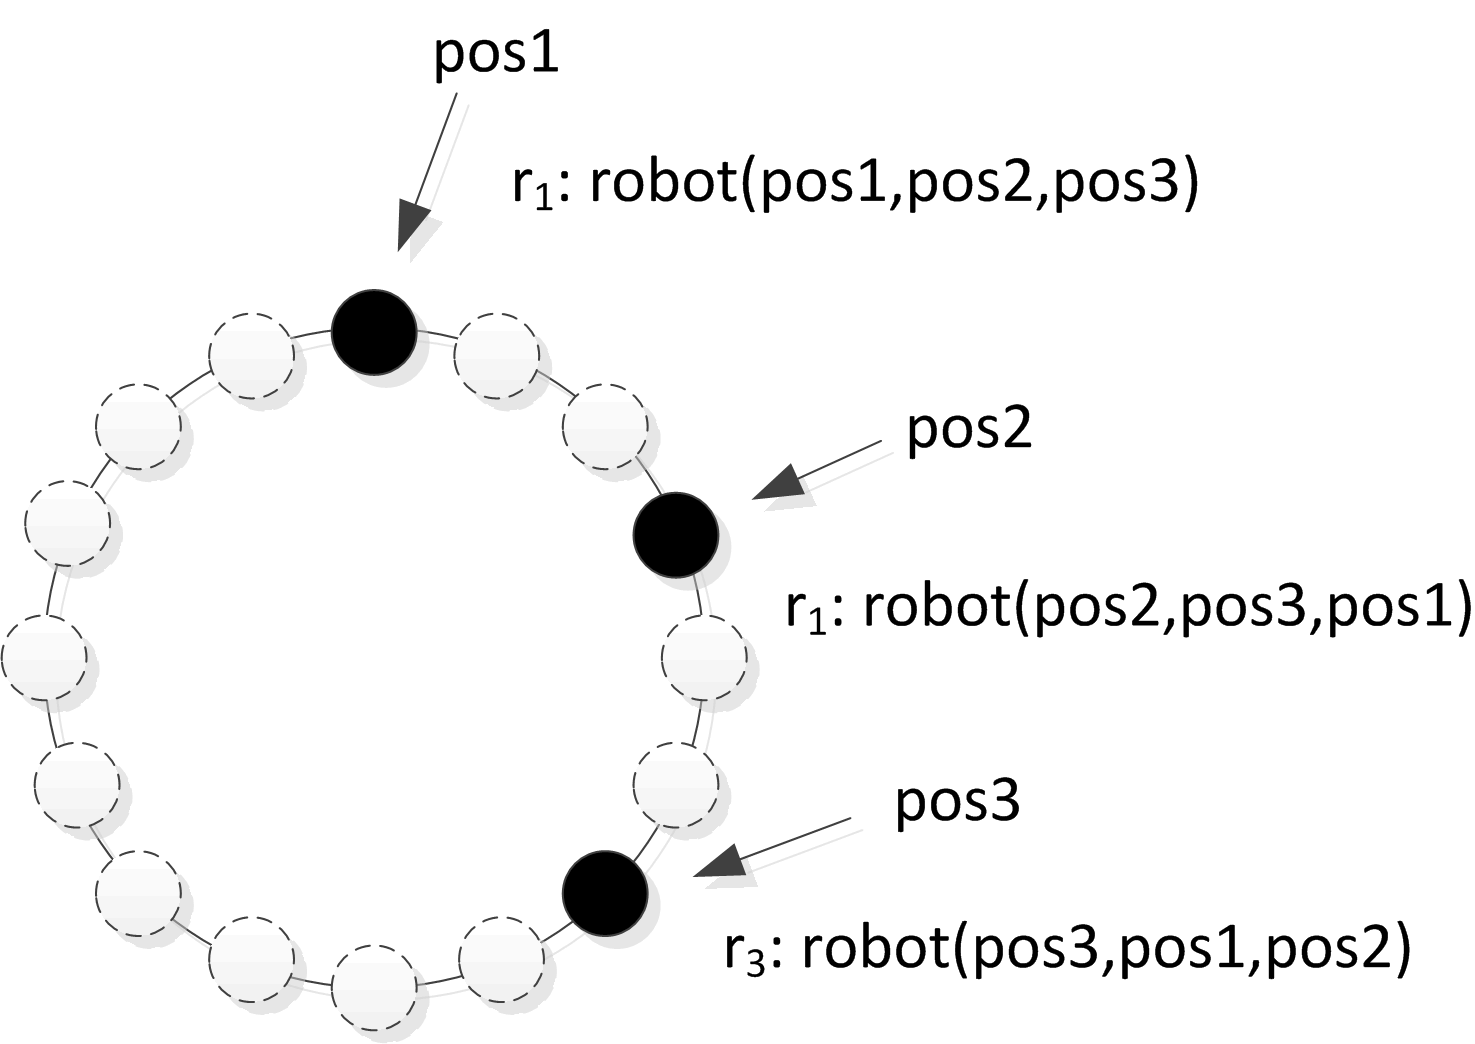
\includegraphics[width=4 in]{fig/params4.png}
	\caption{}
	\label{fig:params4}
\end{figure}

如图\ref{fig:params4},实例化三个机器人$r_1,r_2,r_3$,每个实例化对象的参数列表中第一个变量是当前实例化机器人的位置变量,例如机器人实例$r_1$的第一个参数是$pos1$,机器人实例$r_2$的第一个参数是$pos2$等等。后续参数是按照顺时针传入,例如机器人实例$r_1$中的参数依次是$pos1,pos2,pos3$,机器人实例$r_2$中的参数依次是$pos2,pos3,pos1$,机器人实例$r_3$中的参数依次是$pos3,pos1,pos2$。

\subsection{移动阶段变量}
机器人有三个移动阶段:观察、计算和移动。在模型模型中将观察和计算阶段合并称为观察-计算阶段\verb|(Look-Compute)|,在机器人模型中使用符号\verb|lc|表示,移动阶段使用符号\verb|m|表示。机器人模型中声明机器人移动阶段状态变量为\verb|phase|,\verb|phase|的值域为$\left\{lc,m\right\}$。在nuXmv中\verb|phase| 的具体定义如下:

\begin{lstlisting}
VAR
   phase : {lc,m};

ASSIGN
   init(phase) := lc;
   next(phase) :=
         case
            phase = lc     :  m;
            phase = m      :  lc;
            TRUE           :  phase;
         esac;
\end{lstlisting}

在代码中声明移动阶段变量\verb|phase|,并描述其值域范围为$\left\{lc,m\right\}$。使用$init\left(phase\right)$对变量\verb|phase|进行初始化为\verb|lc|。 使用$next\left(phase\right)$定义移动阶段变量的状态变化:当机器人处于观察-计算阶段\verb|(lc)|时,它的下一个状态为移动阶段\verb|(m)|;当机器人处于移动阶段\verb|(m)|时,下一个状态为观察-计算阶段\verb|(lc)|;\verb|TRUE : phase|表示机器人不是观察-计算阶段和移动阶段时,下一个状态时移动阶段变量的值和当前状态的值一样,保持不变。

\subsection{移动变量}
在机器人模型中声明移动变量,表示机器人在观察-计算阶段获取的移动量。在模型中声明整型变量\verb|move|,表示机器人移动量。在环形空间中,机器人的移动有三种情况:顺时针移动,逆时针移动和不移动。模型中移动量使用整数表示,\verb|1|表示机器人顺时针移动,\verb|-1|表示机器人逆时针移动,\verb|0|表示机器人不移动。所以移动变量\verb|move|的值域范围是$\left\{-1,0,1\right\}$。\verb|move|的取值是机器人通过获取的快照与移动算法匹配进行判定的,具体的判定过程在移动算法建模的时候,进行具体描述。\verb|move|在模型的声明如下:

\begin{lstlisting}
VAR
   move  : -1..1;

ASSIGN
   init(move) := 0;
   next(move) :=
   ...
\end{lstlisting}

建模代码中声明了移动变量\verb|move|,\verb|-1..1|表示其值域范围为$\left\{-1,0,1\right\}$。$next\left(move\right)$表示机器人的下一个状态时的移动量,这里移动量是由机器人移动算法决定的,后续介绍机器人移动算法时,会详细介绍。

\subsection{调度策略变量}
半同步调度策略中只有被调度的机器人才做进行移动操作,模型中使用调度策略变量模拟机器人的调度。在模型中声明一个状态变量名为\verb|dispatcher|,表示调度策略变量。符号\verb|choose|表示机器人被调度,符号\verb|steady| 表示机器人未被调度。所以调度策略变量的值域为$\left\{choose,steady\right\}$。在nuXmv中\verb|dispatcher|的具体定义如下:

\begin{lstlisting}
VAR
   dispatcher : {choose,steady};

ASSIGN
    next(dispatcher) :=
         case
            TRUE     :  {choose,steady};
         esac;
\end{lstlisting}

建模代码中首先声明了调度策略变量\verb|dispatcher|,并指出了\verb|dispatcher|的值域为$\left\{choose,steady\right\}$。代码中未定义\verb|dispatcher| 初始化的值,表明机器人的取值是值域$\left\{choose,steady\right\}$ 当中随机一个,这样可以模拟机器人第一次移动时,是随机调度的。$next\left(dispatcher\right)$表示\verb|dispatcher|的下一个状态时的值,条件分支中只有一个分支$TRUE : \left\{choose,steady\right\}$,\verb|TRUE|表示条件分支永远满足。条件分支的值为$\left\{choose,steady\right\}$,表示下一个状态时,机器人的调度是$\left\{choose,steady\right\}$当中随机一个。这样每次机器人移动动作之前,都是随机被调度的。

\section{环境快照建模}
前面介绍了模型中空间位置变量,空间位置变量在机器人实例化时,是按照顺时针方向依次传入。这样很容易从位置参数的排列顺序知道机器人在空间中位置相邻关系。通过计算空间中两个相邻机器人之间的间隔空间位置个数,来模拟机器人的环境快照。机器人环境快照分顺时针和逆时针快照,所以计算相邻机器人的间隔空间位置个数也分顺时针和逆时针。假设有两个相邻机器人A和B,从A到B的间隔空间位置个数使用$gap_{A \rightarrow B}^F$表示,其中$F \in \left\{+,-\right\}$ 表示\verb|gap|的计算取值方向,\verb|+| 表示顺时针,\verb|-| 表示逆时针。

\begin{figure}[!hbt]
	\centering
	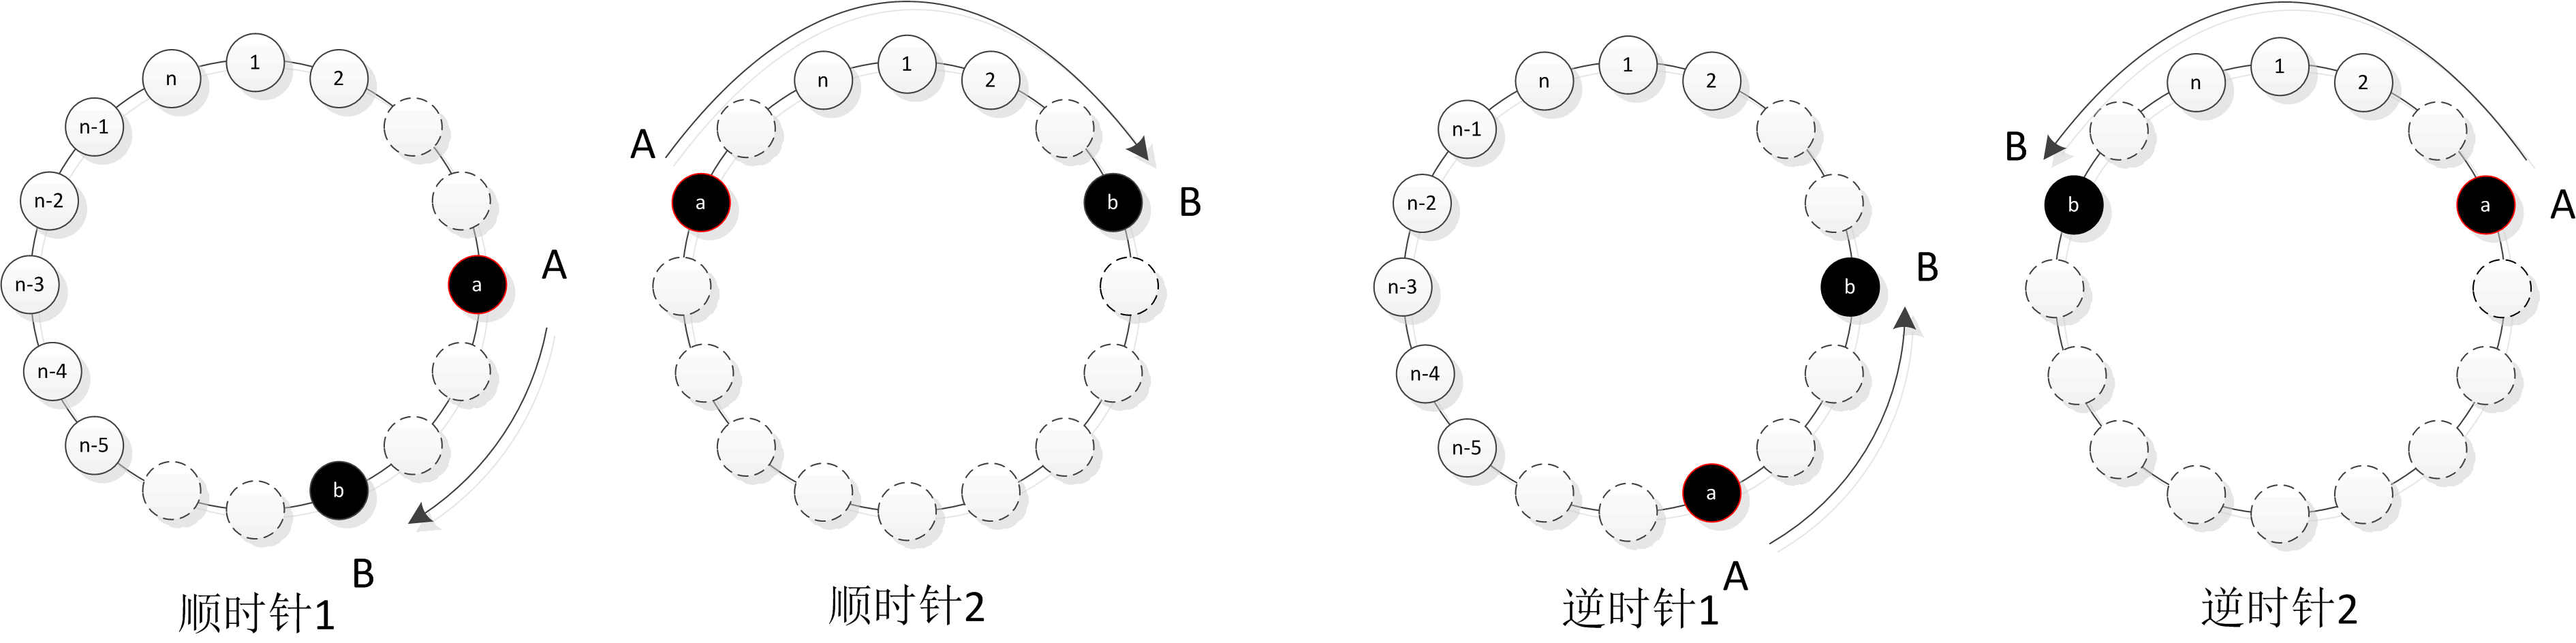
\includegraphics[width=6 in]{fig/gap.png}
	\caption{机器人A和B之间顺时针和逆时针gap计算示意图}
	\label{fig:gap}
\end{figure}

如图\ref{fig:gap}所示,当计算机器人A和B之间的时候,不仅需要考虑顺时针和逆时针方向问题,而且还必须考虑环形空间位置结点编号对空白位置结点个数计算的问题。图中顺时针1求A到B顺时针方向间隔空间位置个数可以使用\verb|b-a| 计算得出。图中顺时针2 从A 到B 顺时针方向间隔空间位置个数,不能简单的使用\verb|b-a| 计算,因为从A到B之间经过了位置结点\verb|n|和\verb|1|。对于逆时针求间隔空间位置个数也有两种情况,图中逆时针1 求A到B顺时针方向间隔空间位置个数可以使用\verb|a-b|计算得出。图中逆时针2 求A 到B顺时针方向间隔空间位置个数也需要考虑位置结点\verb|n|和\verb|1|的问题。通过归纳总结得出计算从A 到B之间间隔空间位置个数的计算公式,如下:

$$gap_{A \rightarrow B}^+ = \left(c \left( B \right) - c \left( A \right) + n\right) \;  mod \; n $$

$$gap_{A \rightarrow B}^- = \left(n - \left( \left( c \left( B \right) -  c \left( A \right) +n\right) \; mod \; n \right) \right) \; mod \; n $$

公式中\verb|n|表示空间环境中空间位置结点的个数。\verb|mod|表示取模运算。下面给出一个具体例子说明机器人的环境快照模型:

\begin{figure}[!hbt]
	\centering
	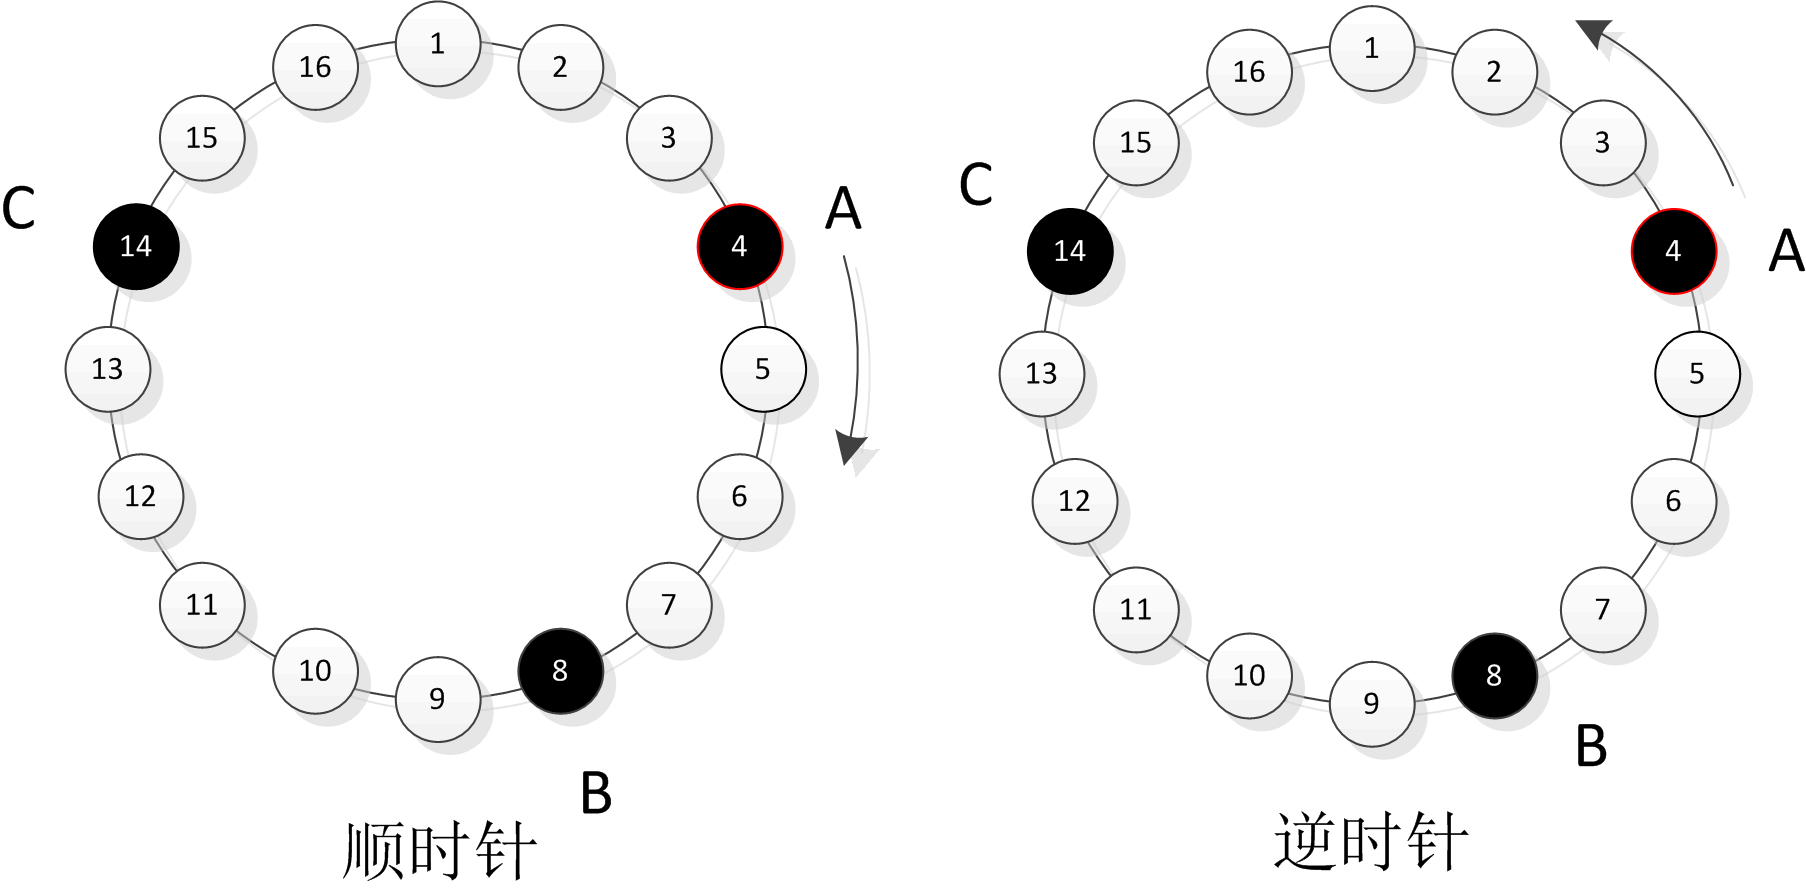
\includegraphics[width=3 in]{fig/gapexpress.png}
	\caption{顺时针和逆时针gap环境快照}
	\label{fig:gapexpress}
\end{figure}

如图\ref{fig:gapexpress}所示,位置结点数为16的环形空间,空间中有三个机器人A、B、C。对于机器人A顺时针方向,使用相邻机器人之间间隔空间位置个数表示环境快照为$\left(4,6,6\right)$,具体计算过程如下:

$$gap_{A \rightarrow B}^+ = \left(8 - 4 + 16\right) \;  mod \; 10 = 4$$

$$gap_{B \rightarrow C}^+ = \left(14 - 8 + 16\right) \;  mod \; 10 = 6$$

$$gap_{C \rightarrow A}^+ = \left(4 - 14 + 16\right) \;  mod \; 10 = 6$$


对于机器人A逆时针方向,使用相邻机器人之间间隔空间位置个数表示环境快照为$\left(6,6,4\right)$,具体计算过程如下:

$$gap_{A \rightarrow C}^- = \left(16 - \left( \left( 14 -  4 + 16\right) \; mod \; 16 \right) \right) \; mod \; 16 = 6 $$

$$gap_{C \rightarrow B}^- = \left(16 - \left( \left( 8 -  14 + 16\right) \; mod \; 16 \right) \right) \; mod \; 16 = 6 $$

$$gap_{B \rightarrow A}^- = \left(16 - \left( \left( 4 -  8  + 16  \right) \; mod \; 16 \right) \right) \; mod \; 16 = 4$$

\section{移动算法建模}
之前介绍了机器人移动算法是由一组一组移动规则组合而成的,而移动规则是环境快照和对应的移动策略构成。在建模过程使用相邻机器人之间间隔空间位置个数表示机器人的环境快照,所以移动算法在建模的时候,也是用同样的建模方式。下面使用最小移动算法中的移动规则RL1作为例子,介绍一下机器人移动算法建模。

$$RL1:\delta_{c\left(r\right)}^F = \left\langle R_2,F_2,R_1,F_{n-5} \right\rangle \rightarrow r.Back$$

移动规则\verb|RL1|中n表示空间中位置个数,将移动规则\verb|RL1|转换成相邻机器人之间间隔空间位置个数的方法表示为:

$$RL1:\delta_{c\left(r\right)}^F = \left(1,3,n-4\right) \rightarrow r.Back$$

假设n=10,那么移动规则RL1的建模如下:

\begin{lstlisting}
  ASSIGN
   next(move) :=
         case
            phase = lc & ((p2 - p1 + 10) mod 10 = 1) & ((p3 - p2 + 10) mod 10 = 3) :  -1;                                           (rule1)
            phase = lc & ((10 - ((p3 - p1 + 10) mod 10)) mod 10 = 1) & ((10 - (p2 - p3 + 10) mod 10) mod 10 = 3) : 1;               (rule2)
            TRUE  :   0;
         esac;
\end{lstlisting}

建模代码中的\verb|move|是前面讲述移动变量,\verb|phase|是移动阶段变量。\verb|next(move)|表示机器人下一个状态时,机器人的移动量。在建模过程移动规则\verb|RL1|拆分为顺时针规则和逆时针规则。\verb|phase = lc|说明只有当机器人处于观察-计算阶段时,才会做机器人的移动量计算。\verb|rule1|表示移动规则\verb|RL1| 的顺时针匹配,\verb|rule2|表示移动规则\verb|RL1|的逆时针匹配。$\left(\left(p2 - p1 + 10\right) mod 10 = 1\right)$机器人的第一个间隙位置个数与移动规则\verb|RL1|中的第一个位置间隙相匹配,即间隙位置个数都是1。\verb|&|在nuXmv中表示与,即所有的间隙位置个数对应相等时,\verb|next(move)|就等于对应的移动量。匹配\verb|rule1|时,移动量为-1,匹配\verb|rule2|时,移动量为1,当不满足上述两种情况时,移动量为0。

假设机器人r的环境快照$\delta_{c\left( r \right)}^F$匹配移动算法中的某条移动规则L,记为$match\left(\delta_{c\left( r \right)}^F,L\right)$。其中规则L可确定的移动方向使用符号$\beta_{\left(L\right)}$ 表示。nuXmv中移动算法建模思想公式如下:

$$ M_{\left(r\right)} = \left\{
\begin{array}{lcl}
1 \quad \, if \left( match \left( \delta_{c\left(r\right)}^F,L\right) \land F=+ \land \beta\left(L\right) = Front\right) \lor \\ \quad \quad  \left(match \left( \delta_{c\left(r\right)}^F,L\right) \land F=- \land \beta\left(L\right) = Back \right) \\
-1 \quad if \left( match \left( \delta_{c\left(r\right)}^F,L\right) \land F=- \land \beta\left(L\right) = Front\right) \lor \\ \quad \quad  \left(match \left( \delta_{c\left(r\right)}^F,L\right) \land F=+ \land \beta\left(L\right) = Back \right) \\
0 \quad \quad  otherwise
\end{array}
\right. $$

公式中$M_{\left(r\right)}$就是移动变量move的值。若机器人\verb|r|在空间位置$c\left(r\right)$的顺时针和逆时针快照对称时$\delta_{c\left(r\right)}^+ = delta_{c\left(r\right)}^-$,若此时机器人r的快照匹配移动算法中某条移动规则L,此时机器人移动量可以是1或者-1。

\section{机器人移动建模}
上面介绍了机器人过程环境快照与移动规则进行匹配,计算获得机器人的移动量move。当机器人处于移动阶段时,机器人会根据移动量move 改变自身的位置。机器人建模中,传入参数\verb|p1|中是当前机器人实例化对象自身的位置。每个机器人移动时,会对应改变\verb|p1|的位置值。具体计算公式如下:

$$ next\left(p1\right) = \left\{
\begin{array}{lcl}
\left(move + p1\right) + n \quad \quad  if \left(move + p1\right) <= 0  \\
\left(move + p1\right)     \quad \quad \quad  if \left(move + p1\right) > 0 \land \left(move + p1\right) <= n \\
\left(move + p1\right) - n \quad \quad  if \left(move + p1\right) > n
\end{array}
\right. $$

其中n表示空间中位置结点个数,计算公式中移动人移动分为三种情况:1、机器人从空间位置1移动到空间位置n,此时移动量move为-1,那么移动之后的机器人所在空间位置为$\left(move + p1\right) + n$。2、机器人不在空间位置1和n 上,此时不需要考虑边界值的问题。1、机器人从空间位置n移动到空间位置1,此时移动量move为1,那么移动之后的机器人所在空间位置为$\left(move + p1\right) - n$。


\section{永恒探索建模}
永恒探索中包含了三条性质:非碰撞性、非互换性和非终止性。在nuXmv中可以使用LTL规格描述三条性质,然后直接在模型中进行验证。下面是使用LTL直接描述三条性质:

\vspace{0.2cm}

\begin{bfseries}非碰撞性(No collision):\end{bfseries}$\ \bigwedge_{i=1}^{k} \bigwedge_{j=1}^{k} \Box \left(i \neq j \rightarrow c_{r_i} \neq c_{r_j}\right)$

\vspace{0.2cm}

\begin{bfseries}非互换性(No switch):\end{bfseries}$$\bigwedge_{h=0}^{n-1}\bigwedge_{i=1}^{k}\bigwedge_{j=1}^{k}  \Box \left(c\left(r_i\right)=h \land  c \left(r_j \right) = \left(h + 1 \right) mod \ n  \rightarrow \ X \ \left( \urcorner  \left(c\left(r_i\right)  = \left(h+1\right) mod \ n \right)   \land c\left(r_j\right) =h \right)\right)$$

\vspace{0.2cm}

\begin{bfseries}非终止性(Live):\end{bfseries}$\ \bigwedge_{h=0}^{n-1} \bigwedge_{i=1}^{k} \Box \Diamond \left(c\left(r_i\right)=h\right)$。

\vspace{0.2cm}

上述公式中n表示空间位置结点个数,k表示空间中的机器人数。在完全异步调度策略中,机器人模块中需要设置公平性,使用LTL描述如下:

\vspace{0.2cm}

\begin{bfseries}公平性(Fairness):\end{bfseries}$\bigwedge_{i=1}^{k} \Box \Diamond \left(r_i.running = true\right)$。

\vspace{0.2cm}

环形空间位置结点个数n=10,机器人数k=3时,使用LTL规格描述机器人任意初始位置、非冲撞性、非互换性和非终止性,实例如下:

\paragraph{任意初始位置}
pos1、pos2、pos3是三个机器人的位置变量,在模型中设定三个机器人在环形空间中的初始位置是按照顺时针排列。那么pos1、pos2、pos3 初始值有三种可能的关系:$1 pos3 \ge pos2 \ge pos3$;$2pos1 \ge pos3 \ge pos2$;$3 pos2 \ge pos1 \ge pos3$。在LTL规则中描述如下:

\begin{lstlisting}
((pos3 > pos2) & (pos2 > pos1)) | ((pos1 > pos3) & (pos3 > pos2)) | ((pos2 > pos1) & (pos1 > pos3)))
\end{lstlisting}

在nuXmv中只限制了机器人位置的初始关系,没有具体指定机器人位置值时,机器人在空间中的位置是任意的,只受到初始关系的约束。

\begin{lstlisting}
/* 非碰撞性 */
LTLSPEC  (((pos3 > pos2) & (pos2 > pos1)) | ((pos1 > pos3) & (pos3 > pos2)) | ((pos2 > pos1) & (pos1 > pos3)))  ->  (G ((pos1 != pos2) & (pos2 != pos3) & (pos1 != pos3)))

/* 非互换性 */
LTLSPEC  (((pos3 > pos2) & (pos2 > pos1)) | ((pos1 > pos3) & (pos3 > pos2)) | ((pos2 > pos1) & (pos1 > pos3))) -> G ((((pos1 + 1) mod 10) = pos2) -> (X (((pos2+1) mod 10) != pos1)) & (((pos2 + 1) mod 10) = pos3) -> (X (((pos3+1) mod 10) != pos2)) & (((pos3 + 1) mod 10) = pos1) -> (X (((pos1+1) mod 10) != pos3)))

/* 非终止性 */
LTLSPEC   (((pos3 > pos2) & (pos2 > pos1)) | ((pos1 > pos3) & (pos3 > pos2)) | ((pos2 > pos1) & (pos1 > pos3))) -> (((G F (pos1 = 0)) & (G F (pos1 = 1)) &...& (G F (pos1 = 9))) & ((G F (pos2 = 0)) & (G F (pos2 = 1)) &...& (G F (pos2 = 9))) & ((G F (pos2 = 0)) & (G F (pos2 = 1)) &...& (G F (pos2 = 9))))
\end{lstlisting}

从例子中可以看出,使用LTL规格描述非冲撞性、非互换性和非终止性三个性质是时,设定机器人的初始位置是任意的。

\section{三种调度策略建模}
本小节中把最小移动算法作为建模实例。下面列举半同步调度策略,完全同步调度策略和完全异步调度策略下使用nuXmv的建模代码。详细介绍每种调度策略的建模构思和实现细节。

\subsection{半同步调度策略建模实例}
下面描述的是环形空间位置结点数为10时,最小移动算法在半同步调度策略下的建模。模型中包含两个模块:主模块\verb|main|和机器人模块\verb|robot|。主模块\verb|main|中定义了空间位置变量、机器人实例和LTL规格。空间位置变量和机器人实例部分代码已经省略。机器人模块\verb|robot|包含了移动阶段、调度策略、移动算法等等。

\begin{lstlisting}
MODULE main
   VAR
     pos1 : 1..10;
     ...
     r1 : robot(pos1,pos2,pos3);
     ...
   LTLSPEC  (((pos3 > pos2)&(pos2 > pos1))|((pos1 > pos3) & (pos3 > pos2))|((pos2 > pos1)&(pos1 > pos3)))->(((G F( (r1.dispatcher = choose)&(r1.phase = lc)))&(G F((r2.dispatcher = choose)&(r2.phase = lc)))&(G F((r3.dispatcher = choose)&(r3.phase = lc))))->(G ((pos1 != pos2)&(pos2 != pos3)&(pos1 != pos3))))
                                                                /* 注释 1 */

MODULE robot(p1,p2,p3)
   VAR
     phase : {lc,m};
     move  : -1..1;
     dispatcher : {choose,steady};                              /* 注释 2 */
   ASSIGN
     init(phase)      := lc;
     init(move)       := 0;
     next(dispatcher) :=
         case
            TRUE           :  {choose,steady};                  /* 注释 3 */
         esac;
     next(phase) :=
         case
            phase = lc     :  m;
            ...
         esac;
     next(move) :=
         case
            dispatcher = choose & phase = lc & ((((p2 - p1) >= 0)? (p2 - p1 - 1):(p2 - p1 - 1 + 10)) = 0) & ((((p3 - p2) >= 0)? (p3 - p2 - 1):(p3 - p2 - 1 + 10)) = 2)  :  -1;
            ...
         esac;
     next(p1) :=
         case
            phase = m & (move + p1) <= 0                        : 10 + (move + p1);
            ...
         esac;
\end{lstlisting}

模型中有三处注释代码,\verb|注释 1|处代码描述机器人非碰撞性的LTL规格,LTL规格中包含所有机器人的调度是公平性,如下:

\begin{lstlisting}
(
     (G F ((r1.dispatcher = choose)&(r1.phase = lc)))
    &(G F ((r2.dispatcher = choose)&(r2.phase = lc)))
    &(G F ((r3.dispatcher = choose)&(r3.phase = lc)))
)
\end{lstlisting}

这部分代码表示机器人\verb|r1|、\verb|r2|和\verb|r3|在未来的都会公平的被调度,而不会出现其中某一个机器人永远不会被调度的情况。在半同步调度策略时,机器人模块中需要声明调度变量\verb|dispatcher|,模拟机器人的调度过程,\verb|注释 2|和\verb|注释 1| 处代码是变量\verb|dispatcher|的声明和下一个状态时值。所以在半同步调度策略中,最关键的是机器人调度过程的建模。

\subsection{完全同步调度策略建模实例}
下面描述的是环形空间位置结点数为10时,最小移动算法在完全同步调度策略下的建模。在完全同步调度策略中,所有机器人都会被同步调度,因此在机器人模块中不需要声明调度变量来区分机器人被调度和未被调度。

\begin{lstlisting}
MODULE main
   VAR
     pos1 : 1..10;
     ...
     r1 : robot(pos1,pos2,pos3);
     ...
LTLSPEC  (((pos3 > pos2) & (pos2 > pos1)) | ((pos1 > pos3) & (pos3 > pos2)) | ((pos2 > pos1) & (pos1 > pos3)))  ->  (G ((pos1 != pos2) & (pos2 != pos3) & (pos1 != pos3)))

MODULE robot(p1,p2,p3)
   VAR
     phase : {lc,m};
     move  : -1..1;
   ASSIGN
     init(phase) := lc;
     init(move)  := 0;
     next(phase) :=
         case
            phase = lc     :  m;
            ...
         esac;
     next(move) :=
         case
            phase = lc & ((p2 - p1 + 10) mod 10 = 1) & ((p3 - p2 + 10) mod 10 = 3) :  -1;
            ...
         esac;
     next(p1) :=
         case
            phase = m & (move + p1) <= 0                      : 10 + (move + p1);
            ...
         esac
\end{lstlisting}

完全同步调度策略建模实例中,机器人\verb|r1|、\verb|r2|和\verb|r3|都是同步移动。相对于半同步调度策略建模而言,完全同步调度策略建模中没有定义调度变量,其他部分建模完全相同。


\subsection{完全异步调度策略建模实例}
下面描述的是环形空间位置结点数为10时,最小移动算法在完全异步调度策略的建模。同完全同步调度策略建模作比较,完全异步调度策略建模有两点差别。

\begin{lstlisting}
MODULE main
   VAR
     pos1 : 1..10;
     ...
     r1 : process robot(pos1,pos2,pos3);                              /* 注释 4 */
     r2 : process robot(pos2,pos3,pos1);
     r3 : process robot(pos3,pos1,pos2);
  LTLSPEC  (((pos3 > pos2) & (pos2 > pos1)) | ((pos1 > pos3) & (pos3 > pos2)) | ((pos2 > pos1) & (pos1 > pos3)))  ->  (G ((pos1 != pos2) & (pos2 != pos3) & (pos1 != pos3)))

MODULE robot(p1,p2,p3)
   VAR
     phase : {lc,m};
     move  : -1..1;
   ASSIGN
     init(phase) := lc;
     init(move)  := 0;
     next(phase) :=
         case
            phase = lc     :  m;
            phase = m      :  lc;
            TRUE           :  phase;
         esac;
     next(move) :=
         case
            phase = lc & ((p2 - p1 + 10) mod 10 = 1) & ((p3 - p2 + 10) mod 10 = 3) :  -1;
            ...
         esac;
     next(p1) :=
         case
            phase = m & (move + p1) <= 0                      : 10 + (move + p1);
            ...
         esac;
     FAIRNESS                                                 /* 注释 5 */
       running
\end{lstlisting}

注释4是机器人实例化代码,机器人实例\verb|r1|,\verb|r2|和\verb|r3|被关键词\verb|process|修饰,说明三个机器人是异步的。注释5定义机器人移动的公平性。完全异步调度策略建模中,关键是需要描述机器人移动的异步性和公平性。


\section{本章小结}
在本章节中,提出了使用符号模型检测工具\verb|nuXmv|实现对机器人和探索算法的建模方法。并且以最小移动算法为例,使用\verb|nuXmv|的基本数据类型定义机器人的属性,如空间位置、移动阶段、移动量和调度。使用\verb|nuXmv|参数化模块定义了机器人模型,在机器人模型中定义了机器人的移动算法。使用LTL规格描述了非碰撞性、非互换性和非终止性。最后,使用举例的方式,分别介绍了半同步调度策略,完全同步调度策略和完全异步调度策略下建模的相同点和不同点。
